\newcounter{case}
\newcommand\case{\stepcounter{case}\arabic{case}}
\chapter{USER INTERFACE DESIGN}
\label{ch:interfaceDesign}%
\section{eMSP Application}

\begin{figure}[H]
    \begin{minipage}[t]{.45\textwidth} % not "0.5\textwidth"
    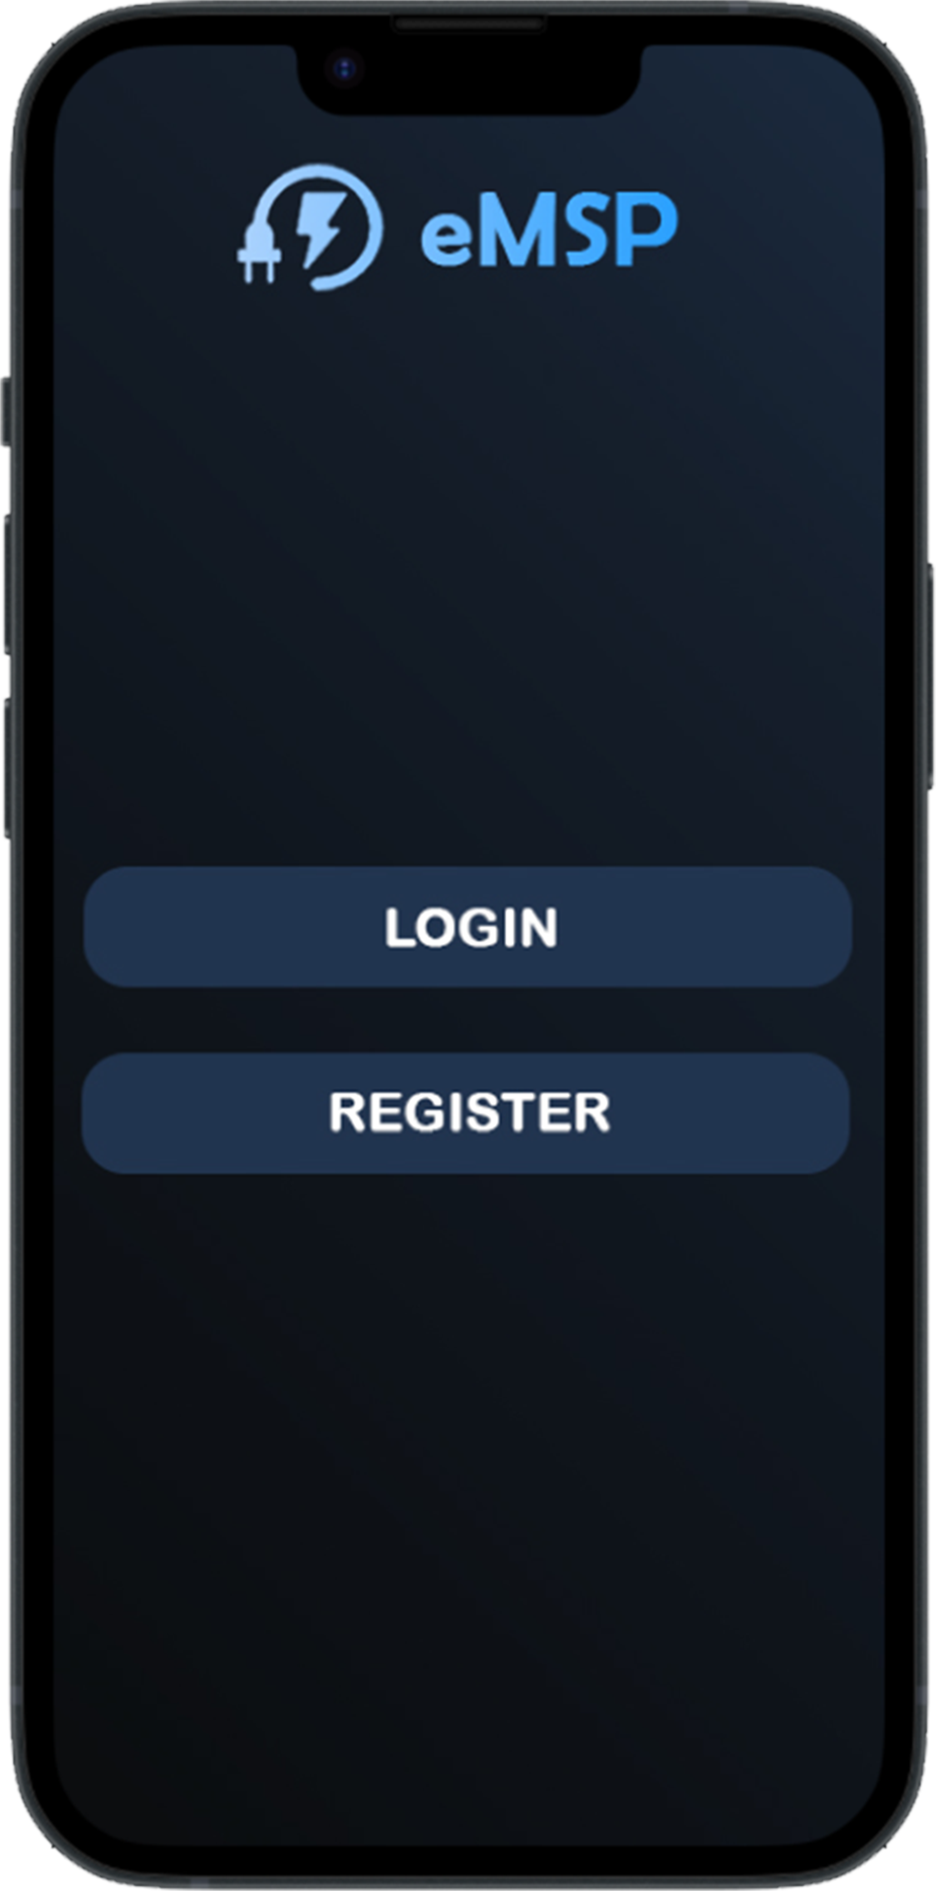
\includegraphics[width=\textwidth]{Mock/eMSP/MainPage}
    \caption{Main Page}
    \label{fig:MainPage}
\end{minipage}
\hfill
\begin{minipage}[t]{.45\textwidth}
    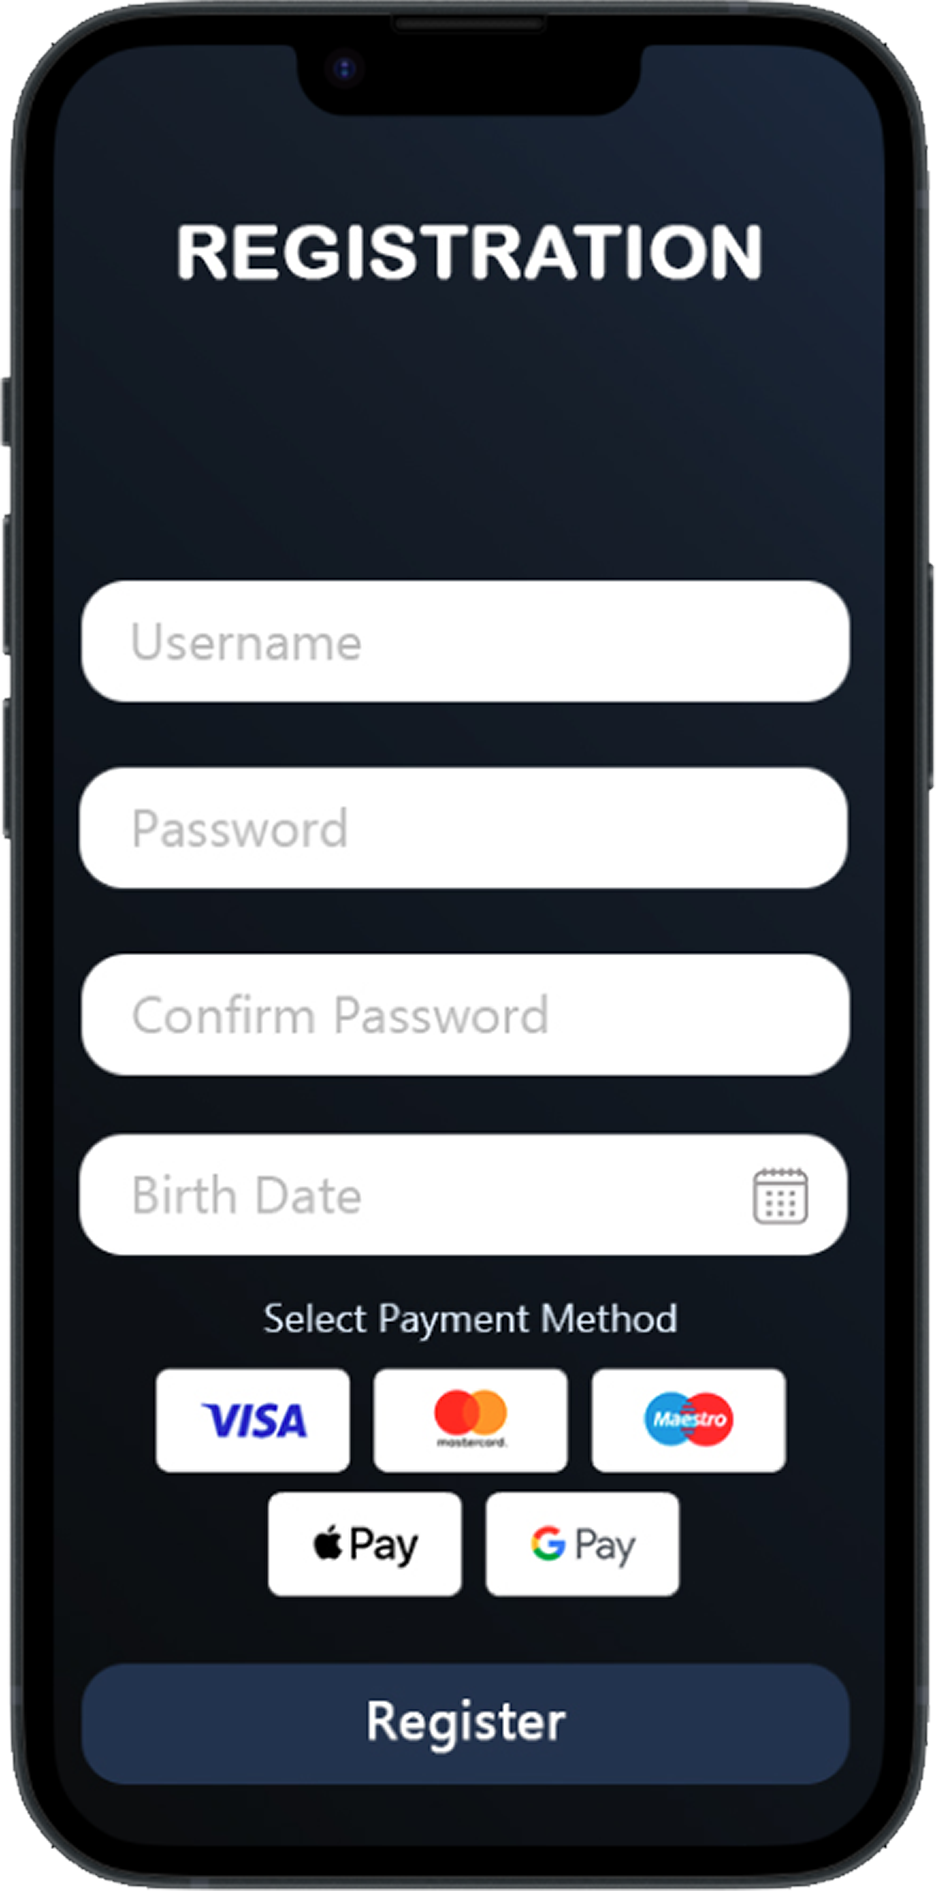
\includegraphics[width=\textwidth]{Mock/eMSP/Registration}
    \caption{Registration Page}
    \label{fig:Registration}
\end{minipage}
\end{figure}
In these two mockups the registration functionality is shown, allowing the user to input his personal data and select a payment method.
\begin{figure}[H]
    \begin{minipage}[t]{.45\textwidth} % not "0.5\textwidth"
    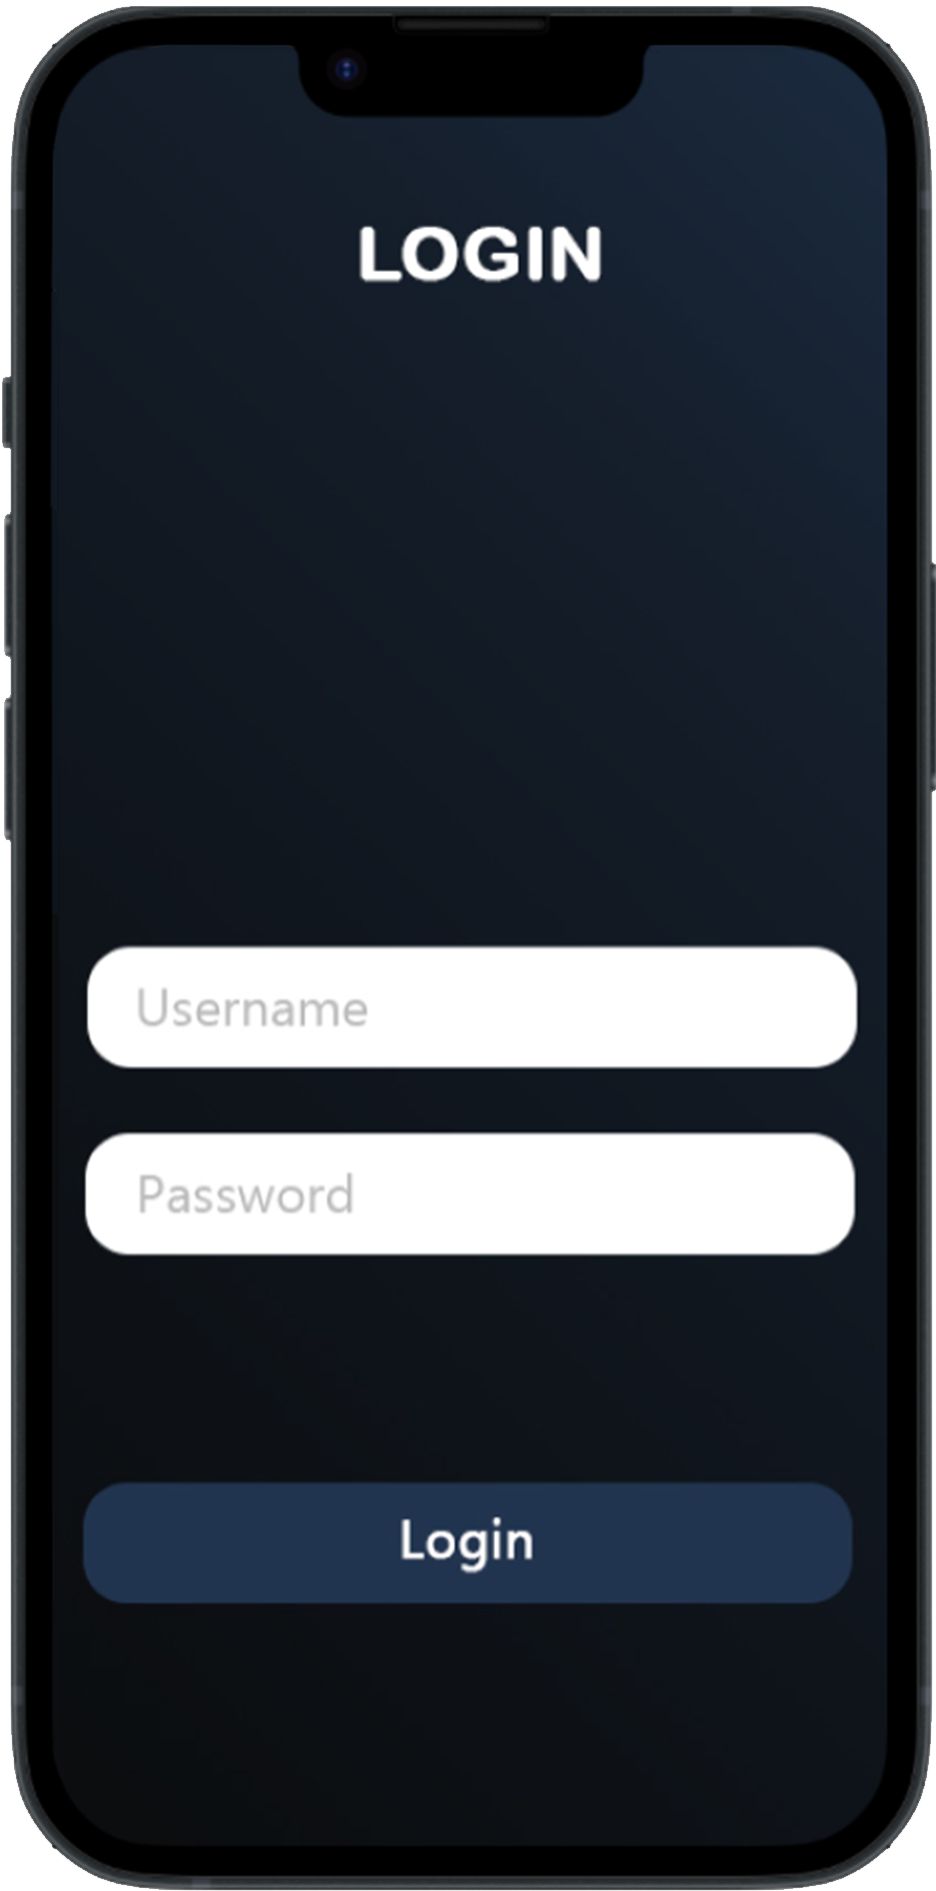
\includegraphics[width=\textwidth]{Mock/eMSP/eMSPLogin}
    \caption{Login Page}
    \label{fig:eMSPLogin}
\end{minipage}
\hfill
\begin{minipage}[t]{.45\textwidth}
    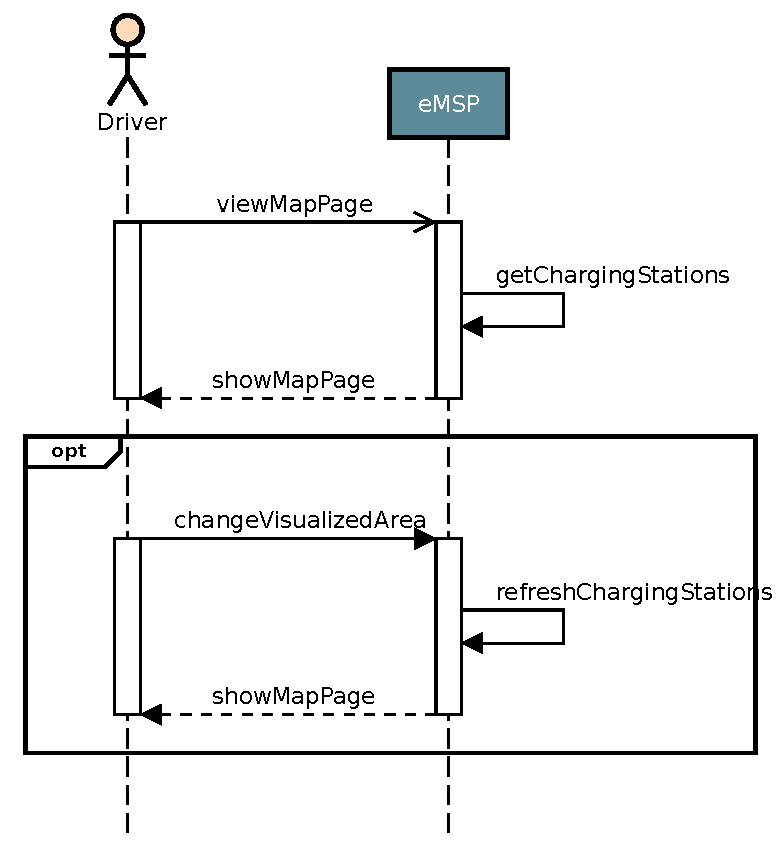
\includegraphics[width=\textwidth]{Mock/eMSP/Map}
    \caption{Map Page}
    \label{fig:Map}
\end{minipage}
\end{figure}
The image on the left shows the login page for the Driver meanwhile, the one on the right shows the main page of the eMSP mobile application, the map page, which allows the Driver to navigate the map, set filters, clicks on station and also access his booking.
\begin{figure}[H]
    \begin{minipage}[t]{.45\textwidth} % not "0.5\textwidth"
    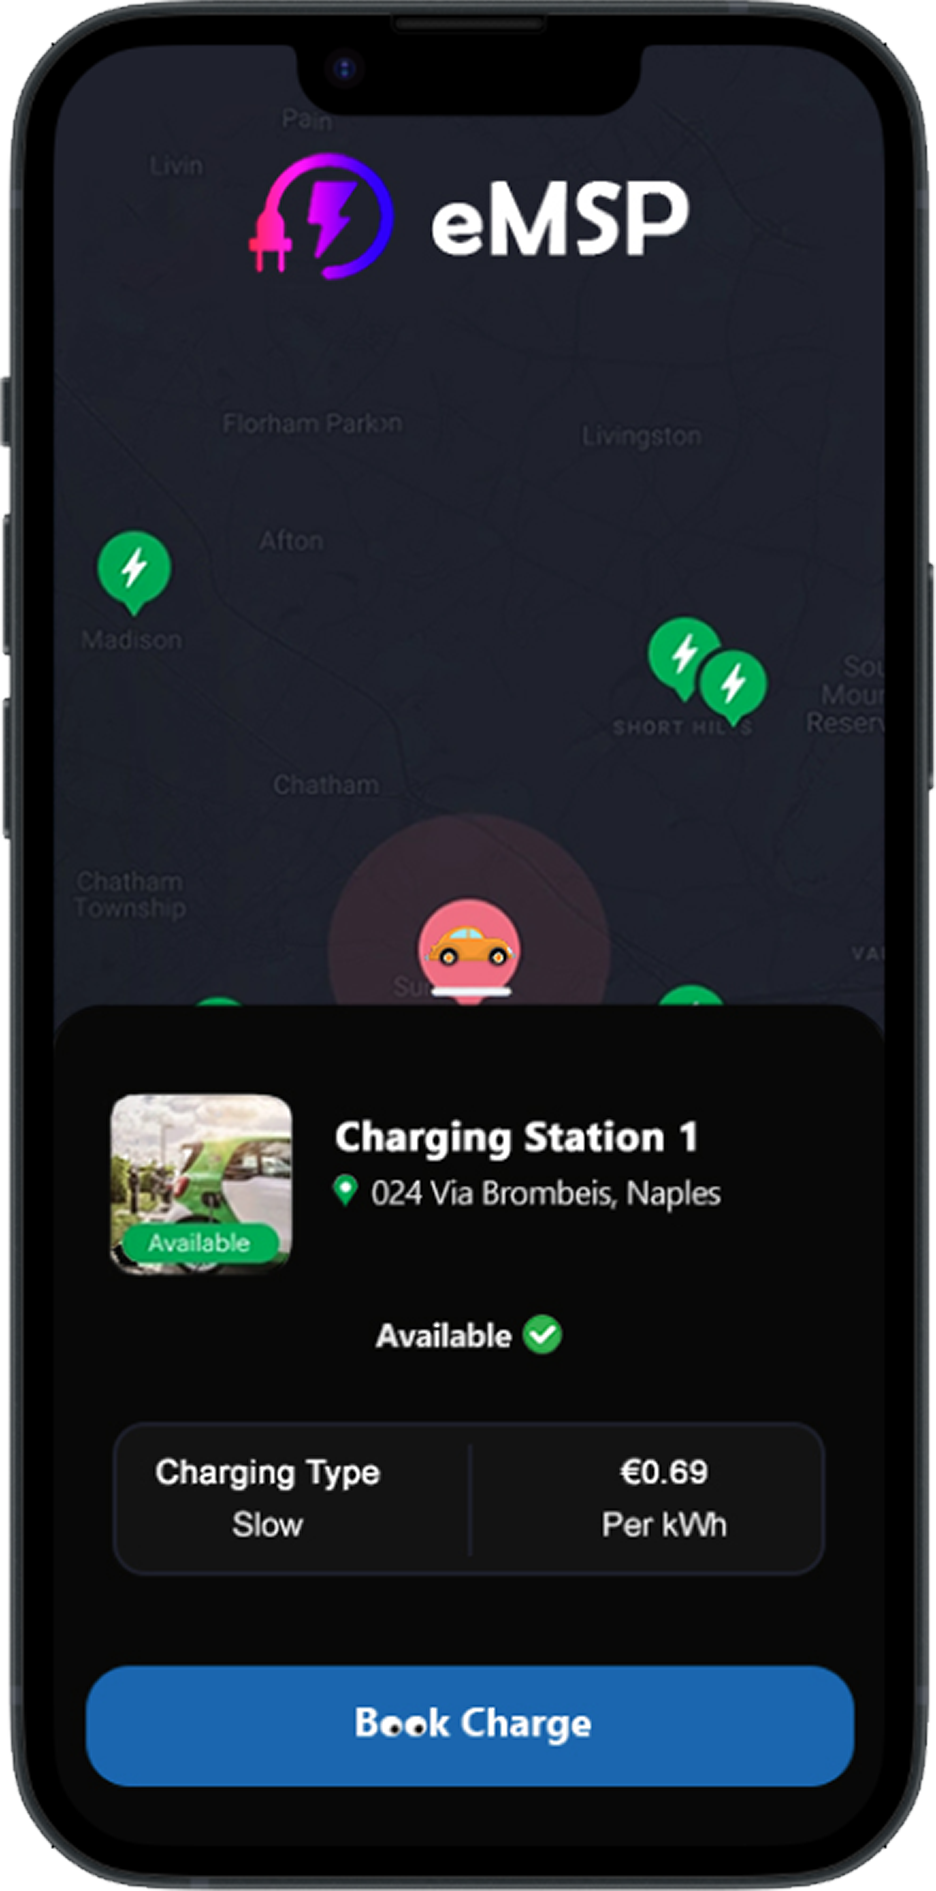
\includegraphics[width=\textwidth]{Mock/eMSP/StationInfo}
    \caption{Charging Station Info Page}
    \label{fig:StationInfo}
\end{minipage}
\hfill
\begin{minipage}[t]{.45\textwidth}
    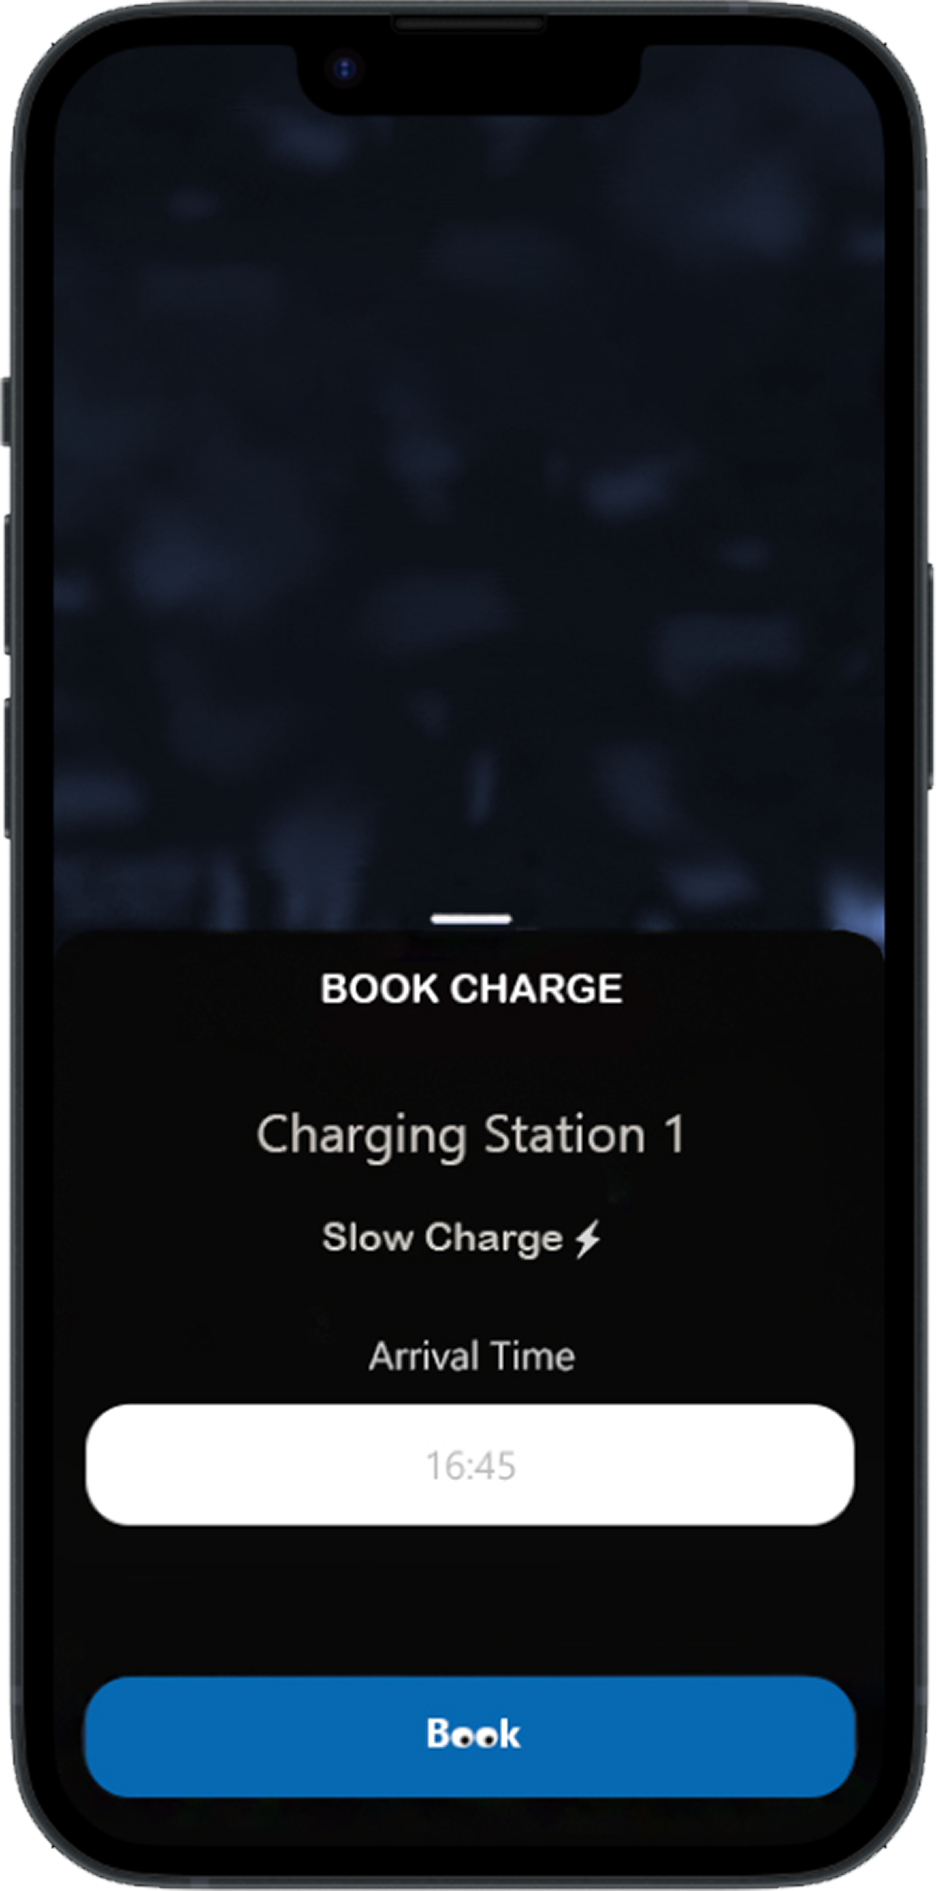
\includegraphics[width=\textwidth]{Mock/eMSP/BookCharge}
    \caption{Book Charge Page}
    \label{fig:BookCharge}
\end{minipage}
\end{figure}
These two mockups show the charging station page, on the left, from which the Driver can see its information and also book a charge for the selected charging type and also set the arrival time.
\begin{figure}[H]
    \begin{minipage}[t]{.45\textwidth} % not "0.5\textwidth"
    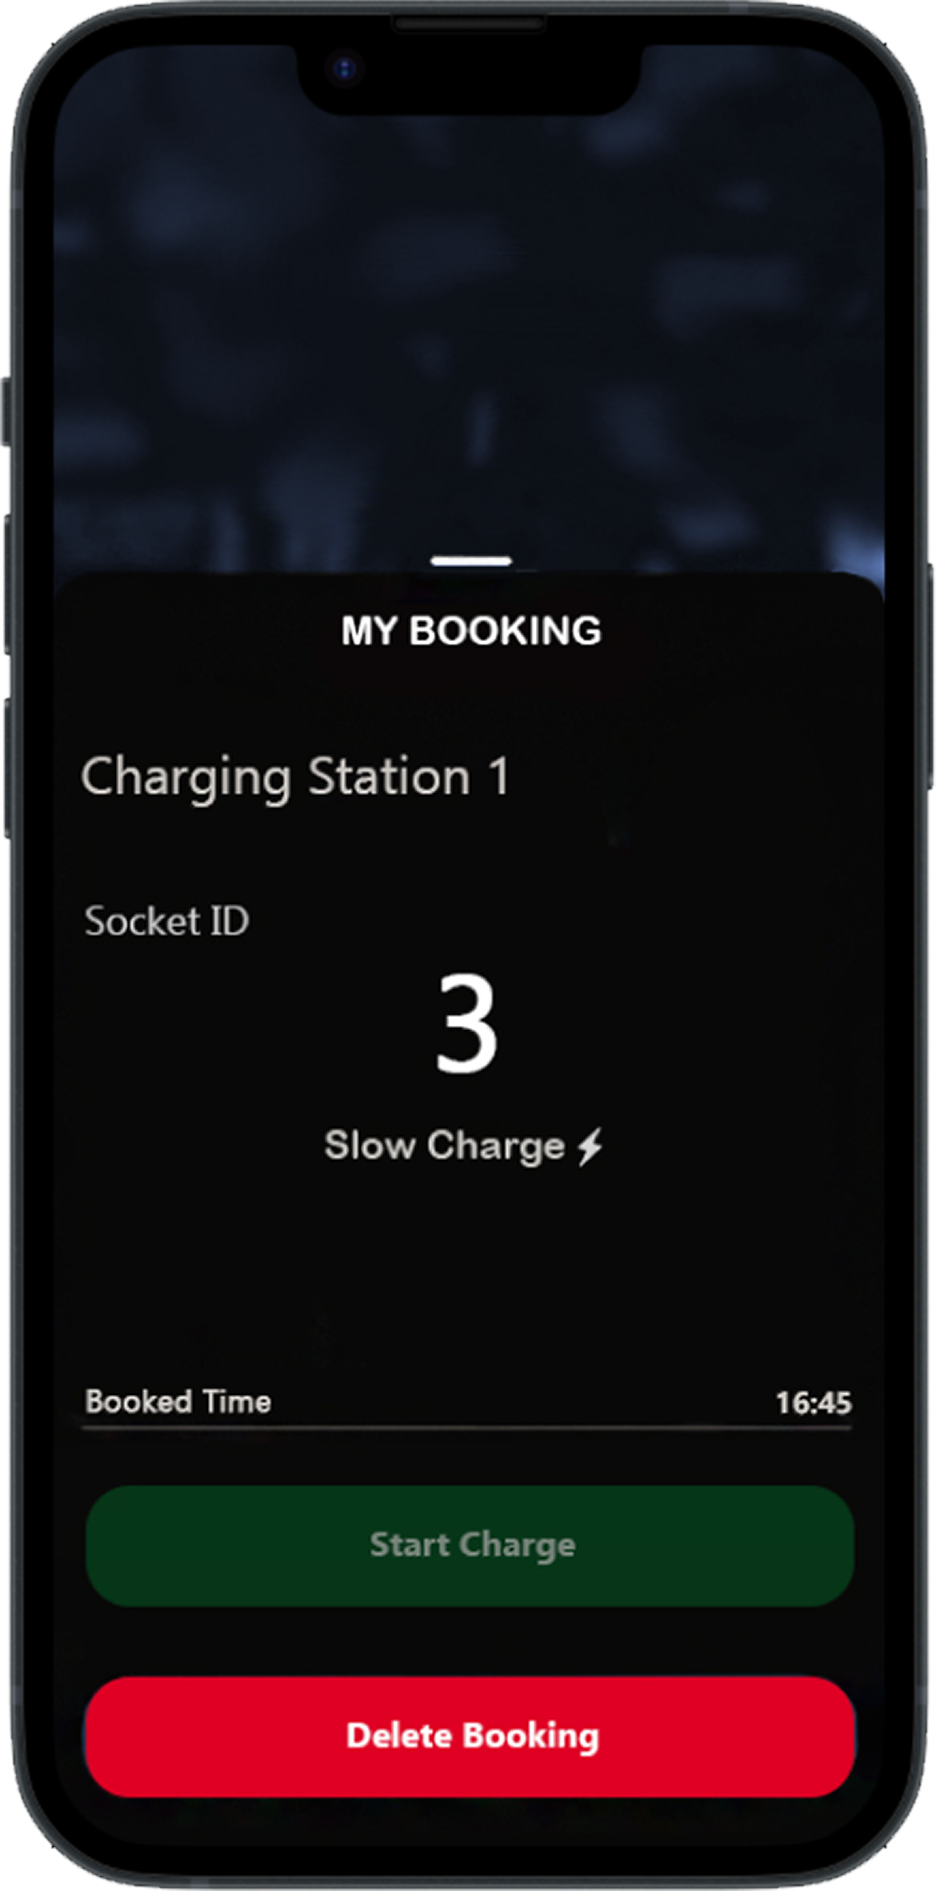
\includegraphics[width=\textwidth]{Mock/eMSP/MyBooking}
    \caption{My Booking Page}
    \label{fig:MyBooking}
\end{minipage}
\hfill
\begin{minipage}[t]{.45\textwidth}
    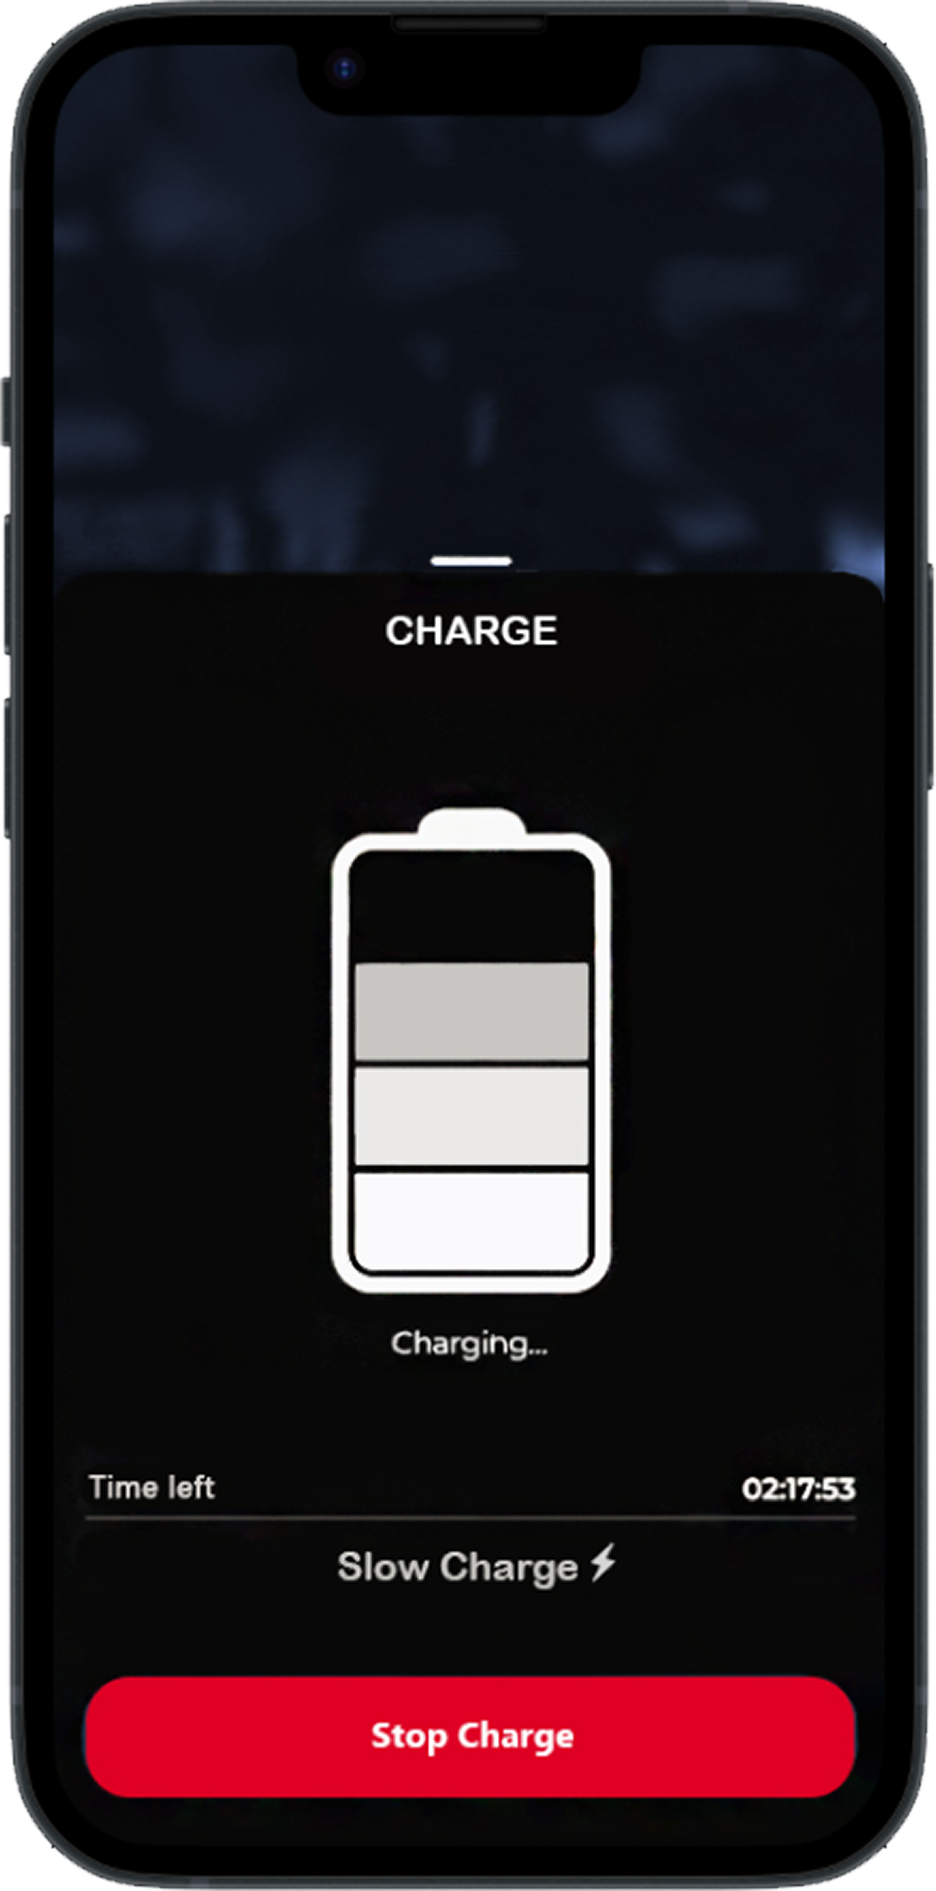
\includegraphics[width=\textwidth]{Mock/eMSP/ChargingProcess}
    \caption{Charging Process Page}
    \label{fig:ChargingProcess}
\end{minipage}
\end{figure}
The mockups show the charging process functionality, which can be initiated from the personal booking page (accessible from the map page). On the right image, the charging view is shown, with the option to interrupt the charging process by pressing the respective button. 
\section{CPMS}

\begin{figure}[H]
    \begin{center}
    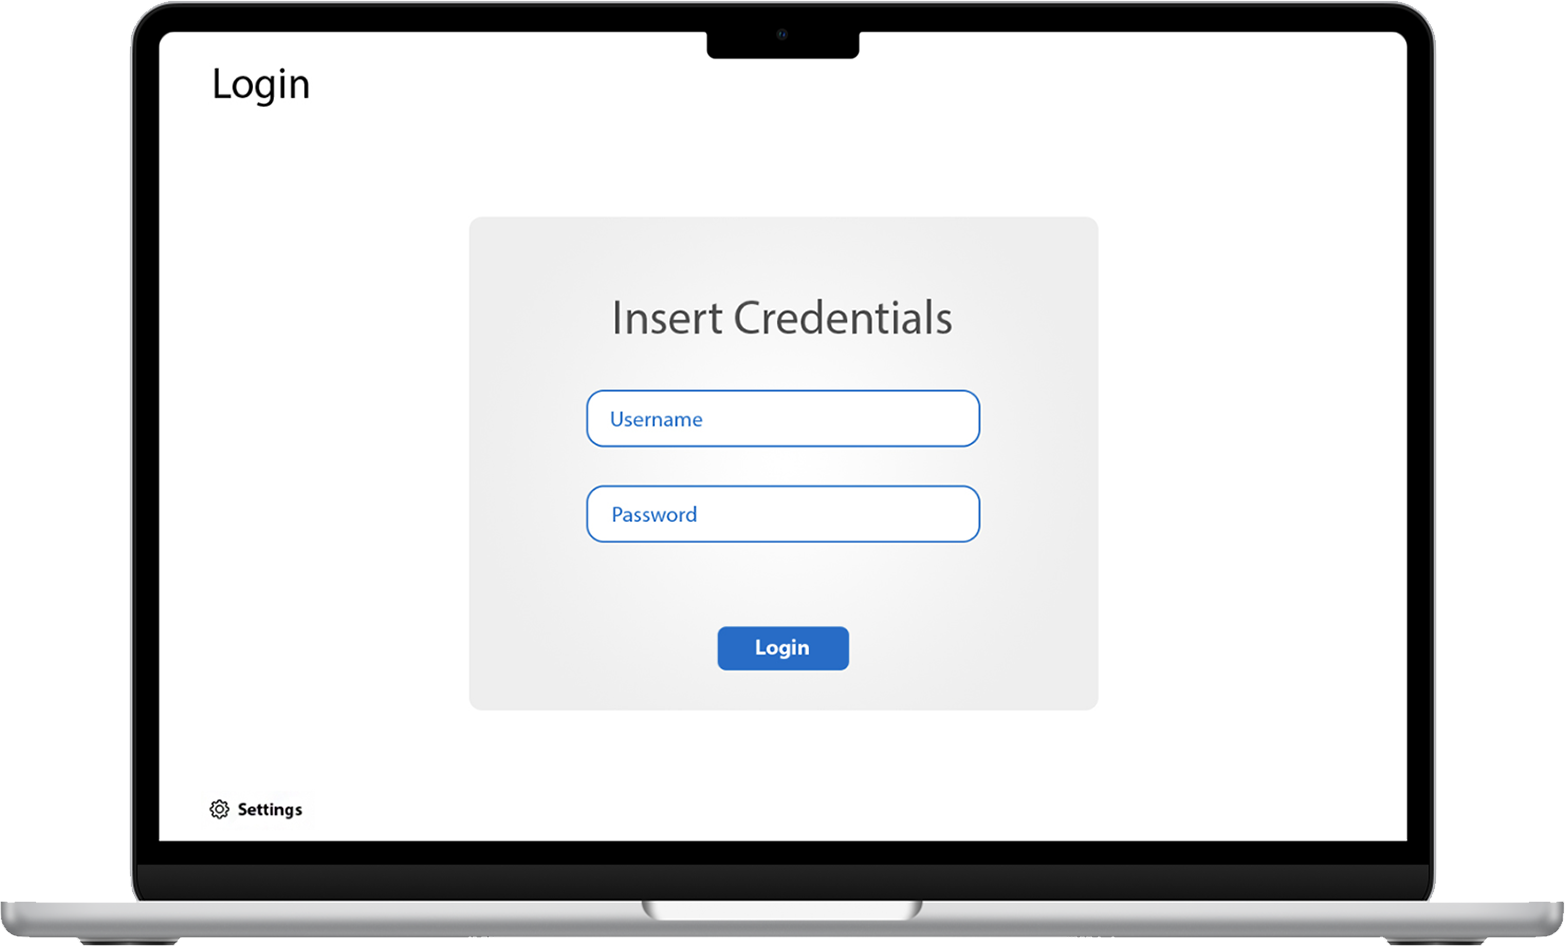
\includegraphics[
        width=\textwidth,
        height=\textheight,
        keepaspectratio]{Mock/CPMS/CPMSLogin}
    \caption{Login Page}
    \label{fig:CPMSLogin}
    \end{center}
\end{figure}
The mockup shows the login page for the CPO.
\begin{figure}[H]
    \begin{center}
    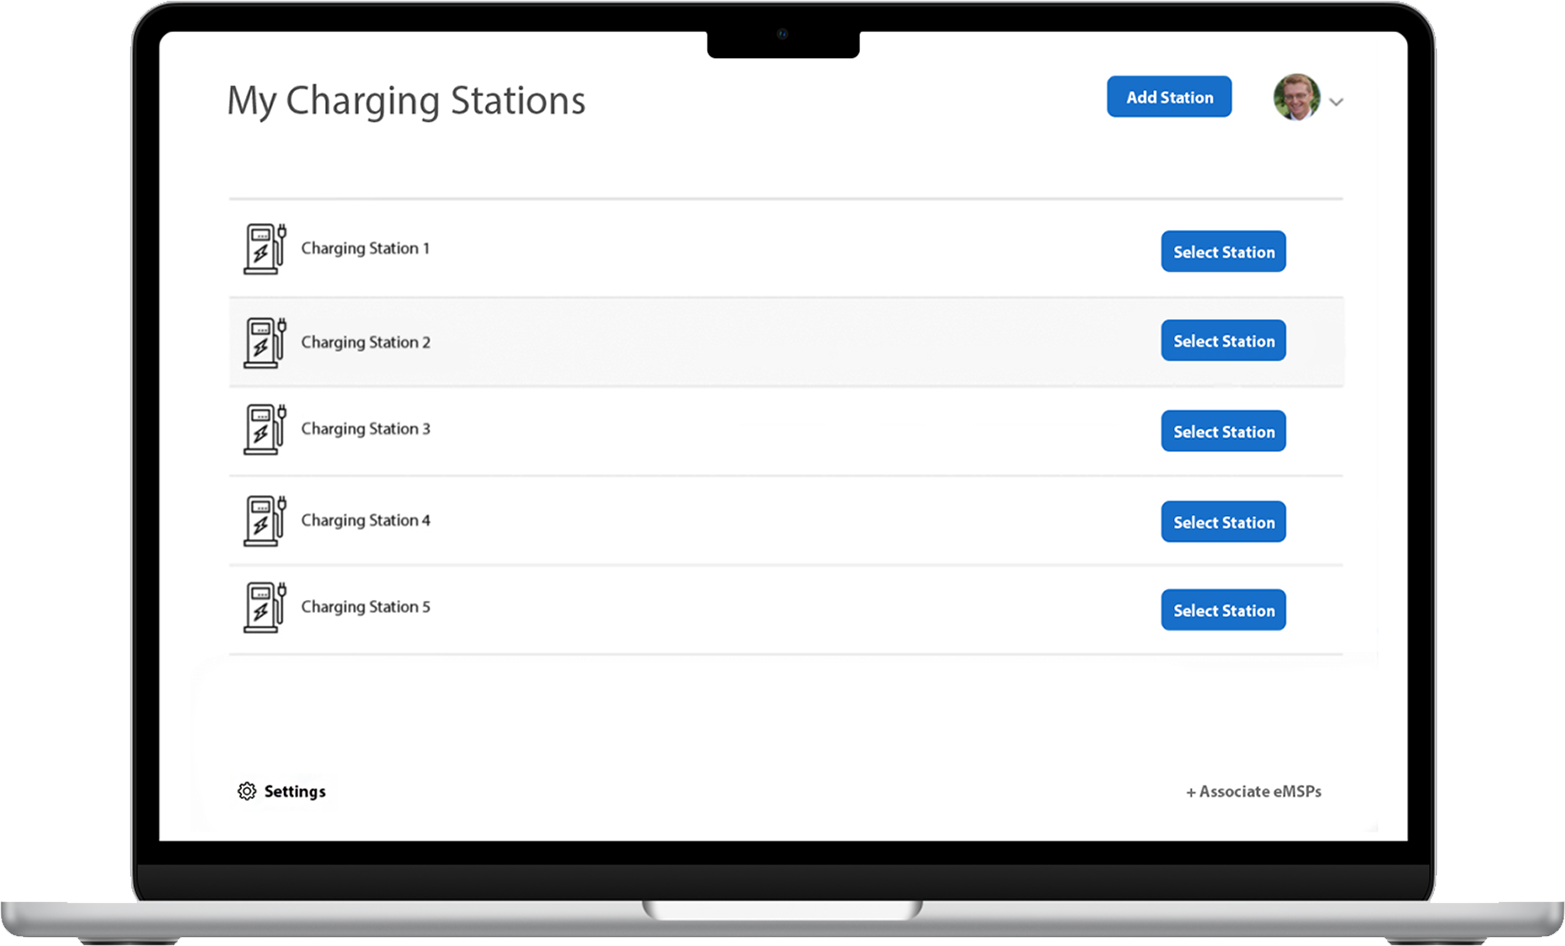
\includegraphics[
        width=\textwidth,
        height=\textheight,
        keepaspectratio]{Mock/CPMS/CPMSHome}
    \caption{Home Page}
    \label{fig:CPMSHome}
    \end{center}
\end{figure}
The mockup shows the home page of the CPMS, from which the CPO can select his managed stations to monitor them, add a new station or associate new eMSPs.
\begin{figure}[H]
    \begin{center}
    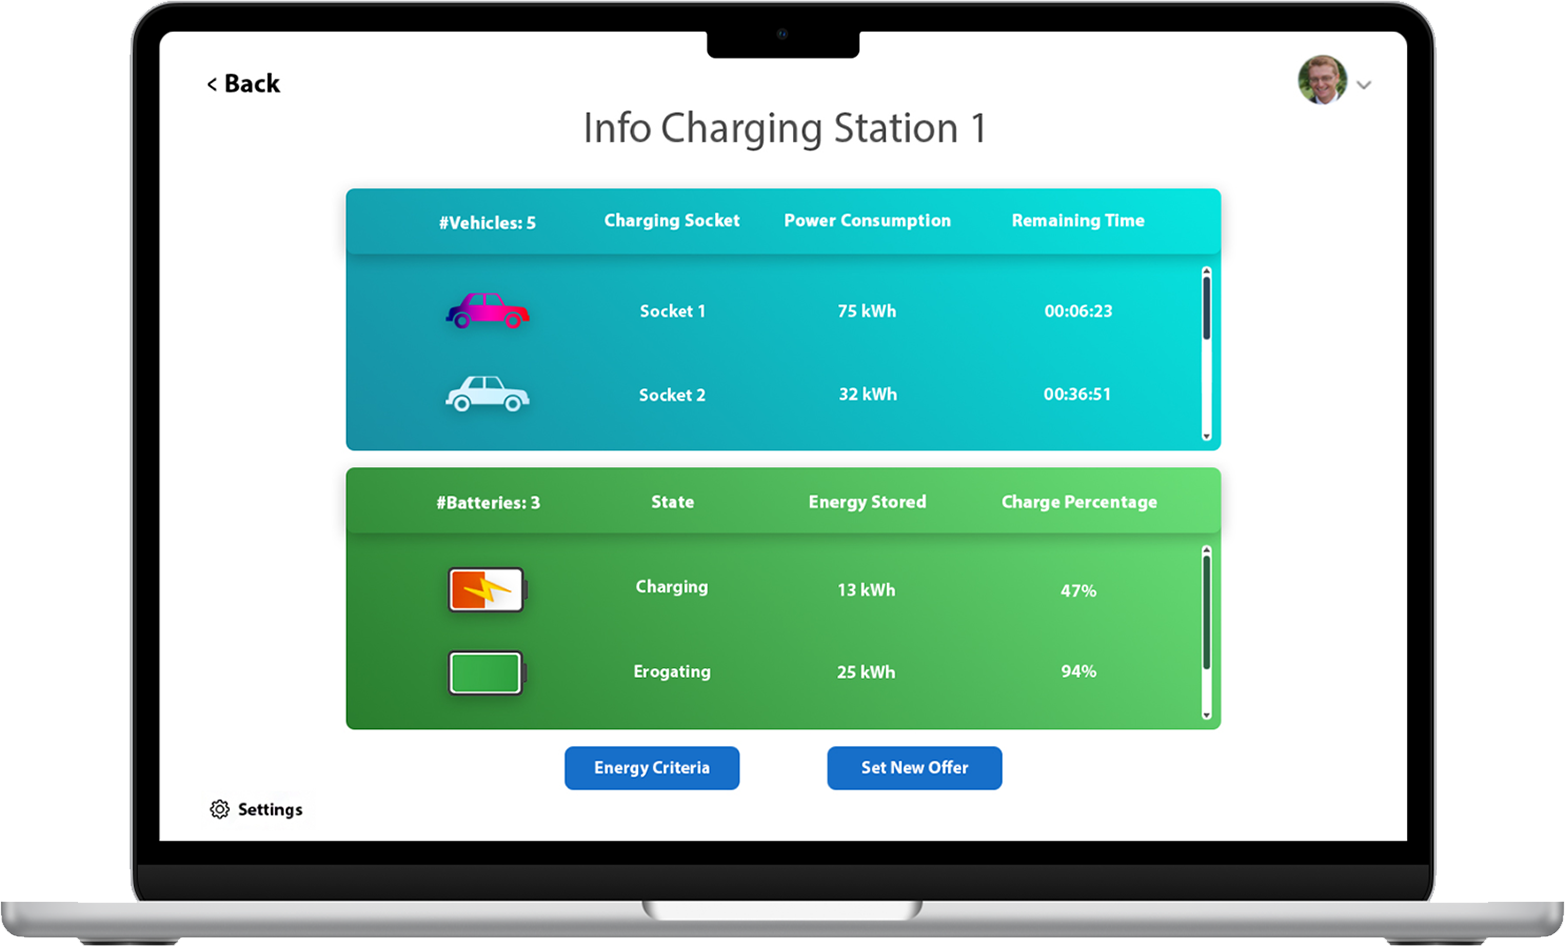
\includegraphics[
        width=\textwidth,
        height=\textheight,
        keepaspectratio]{Mock/CPMS/ChargingStationInfo}
    \caption{Charging Station Info Page}
    \label{fig:ChargingStationInfo}
    \end{center}
\end{figure}
The mockup shows a info page for a charging station, accessible from the main page. here the CPO can see the status of its sockets and batteries. Also, he can update the station's energy criteria and set a new offer.
\begin{figure}[H]
    \begin{center}
    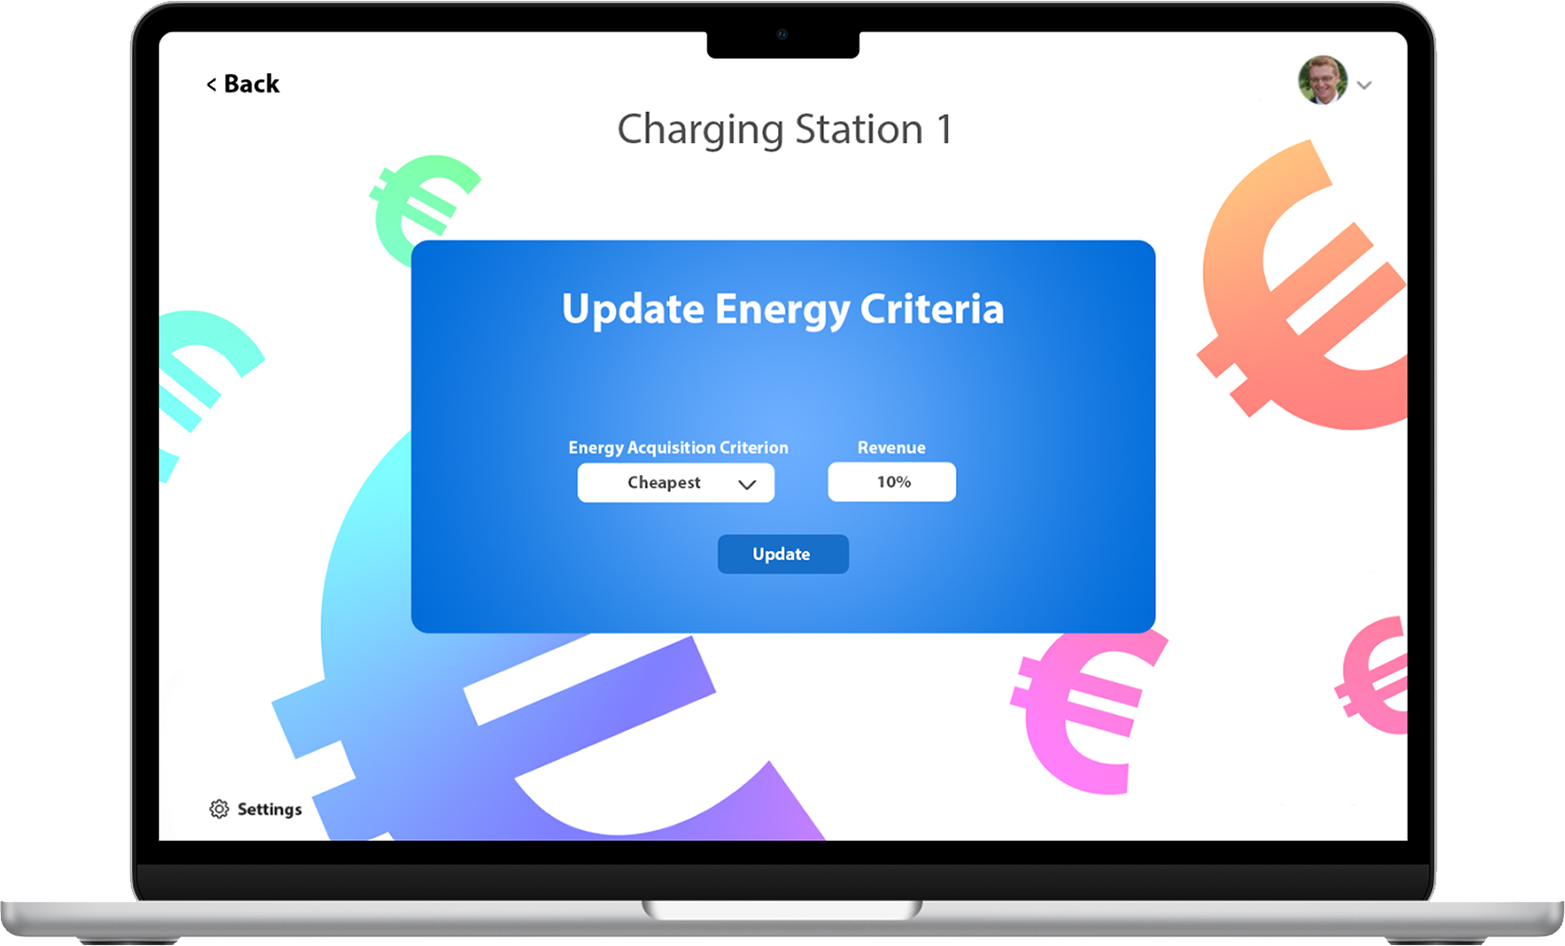
\includegraphics[
        width=\textwidth,
        height=\textheight,
        keepaspectratio]{Mock/CPMS/UpdateCriteria}
    \caption{Update Criteria Page}
    \label{fig:CPMSLogin}
    \end{center}
\end{figure}
The mockup shows the energy criteria page, accessible from the station info page, from which the CPO can update the energy acquisition criteria and the revenue for the selected charging station.
\begin{figure}[H]
    \begin{center}
    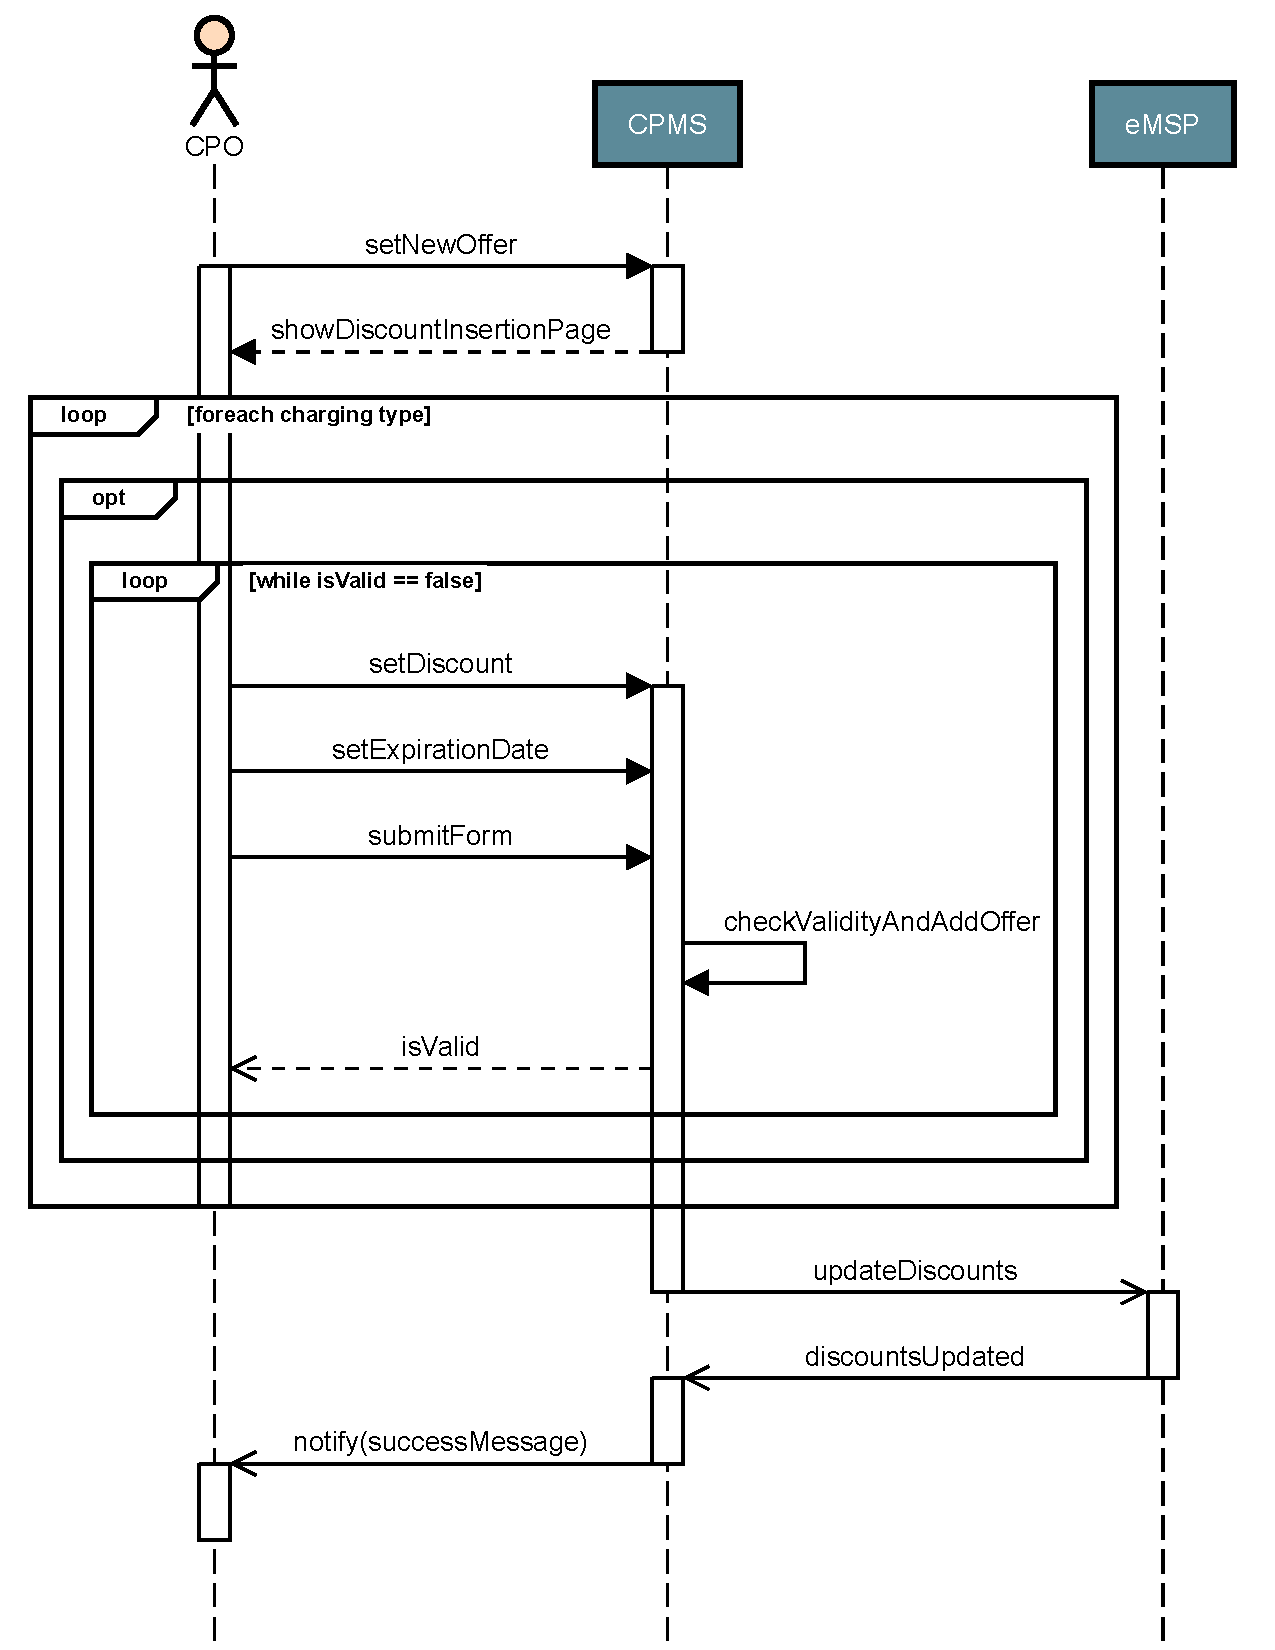
\includegraphics[
        width=\textwidth,
        height=\textheight,
        keepaspectratio]{Mock/CPMS/SetOffer}
    \caption{Set Offer Page}
    \label{fig:SetOffer}
    \end{center}
\end{figure}
The mockup shows the set offer page, accessible from the station info page, from which the CPO can set an offer for each individual charging type and also insert its expiration date.
\begin{figure}[H]
    \begin{center}
    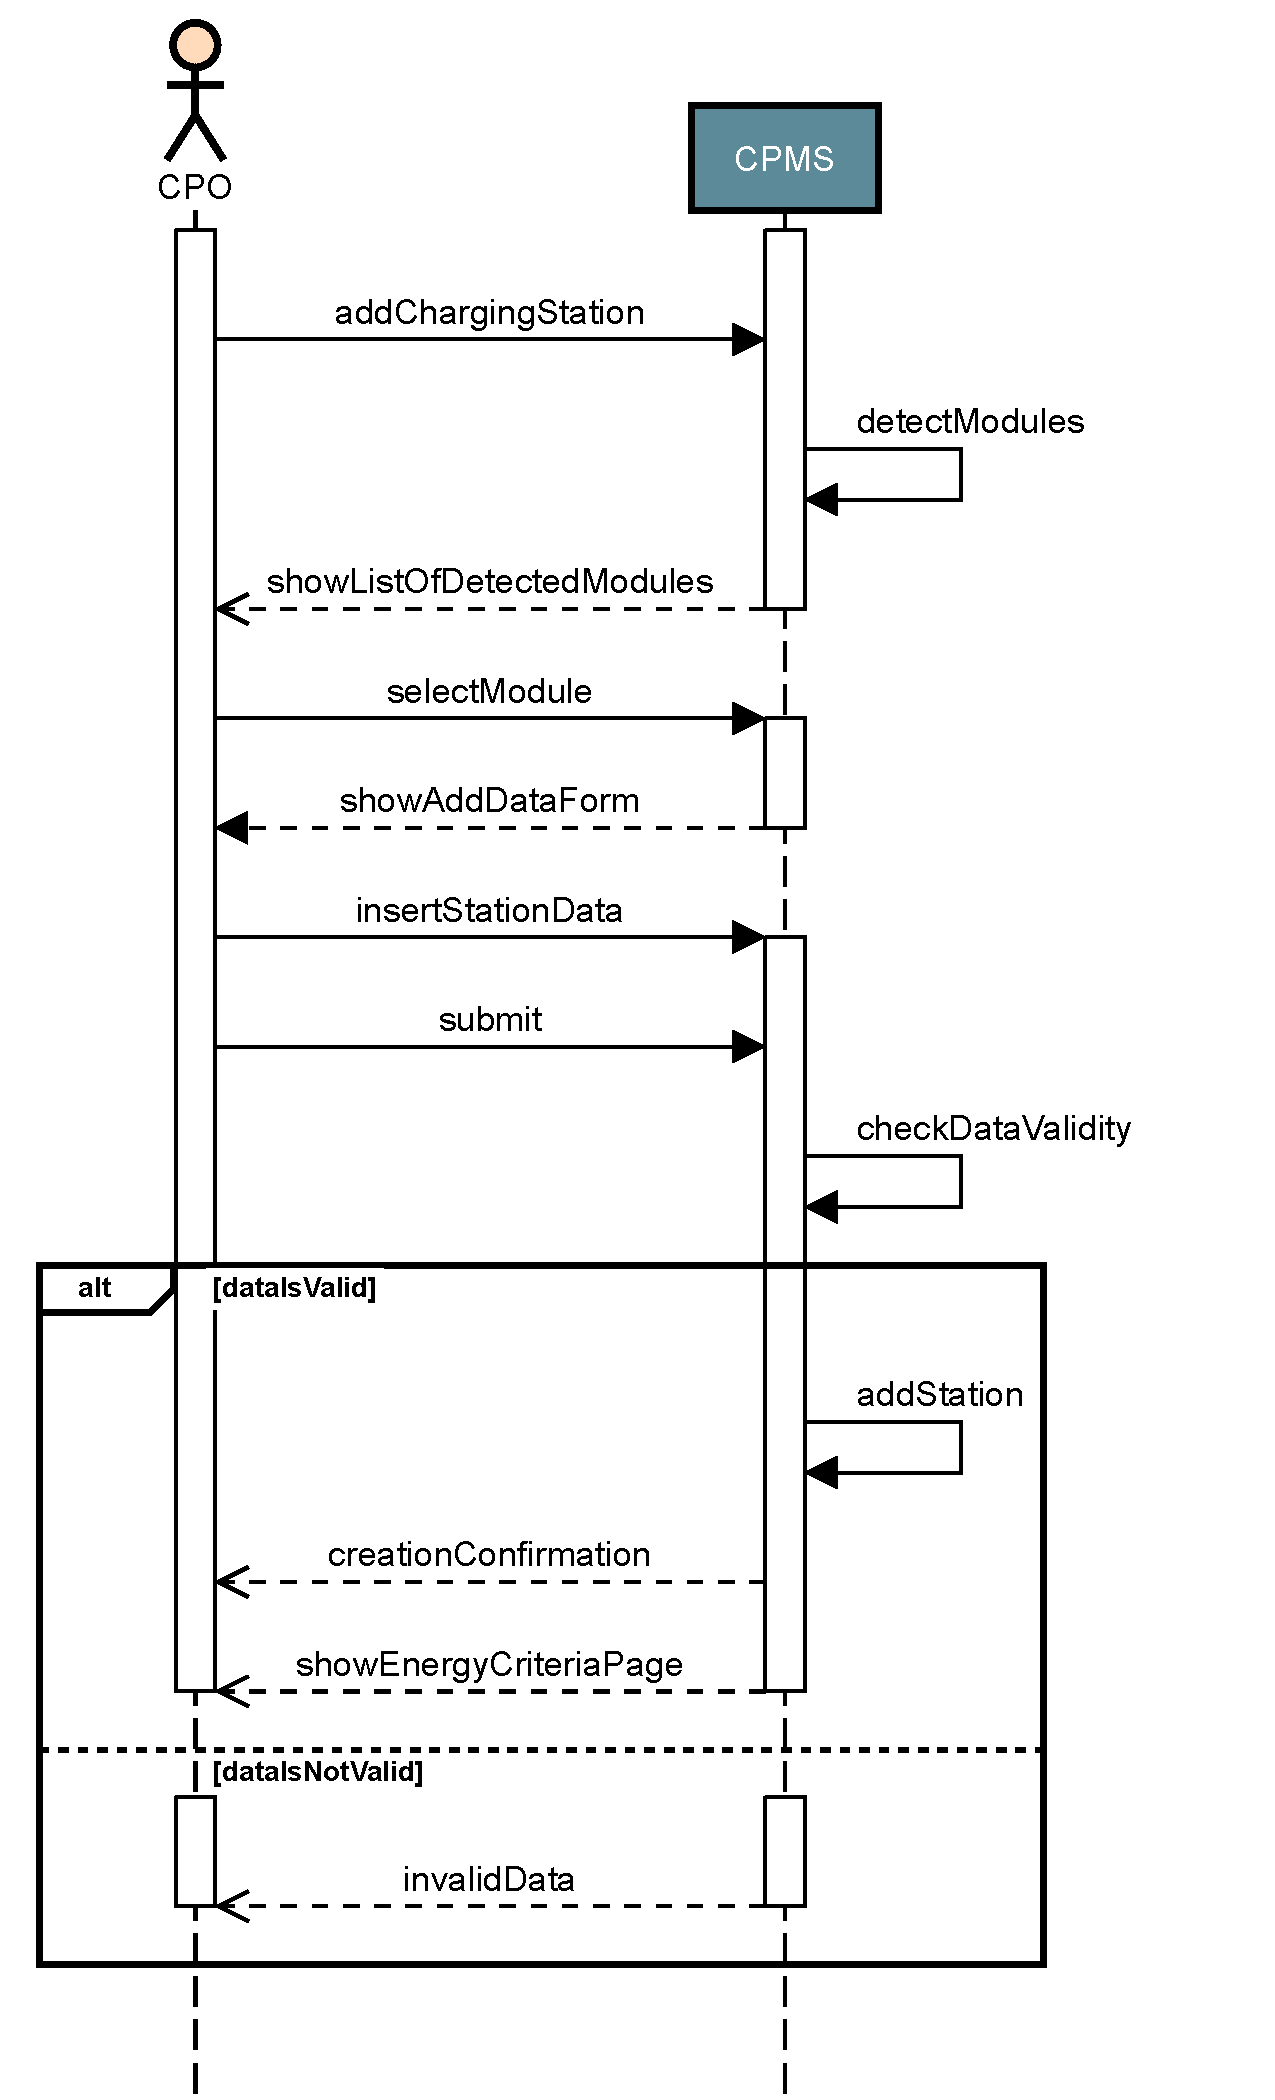
\includegraphics[
        width=\textwidth,
        height=\textheight,
        keepaspectratio]{Mock/CPMS/AddStation}
    \caption{Add Station Page}
    \label{fig:AddStation}
    \end{center}
\end{figure}
The mockup shows the add station page, accessible from the main page, from which the CPO can add a new detected charging station, inserting its name, location and supported charging types.
\begin{figure}[H]
    \begin{center}
    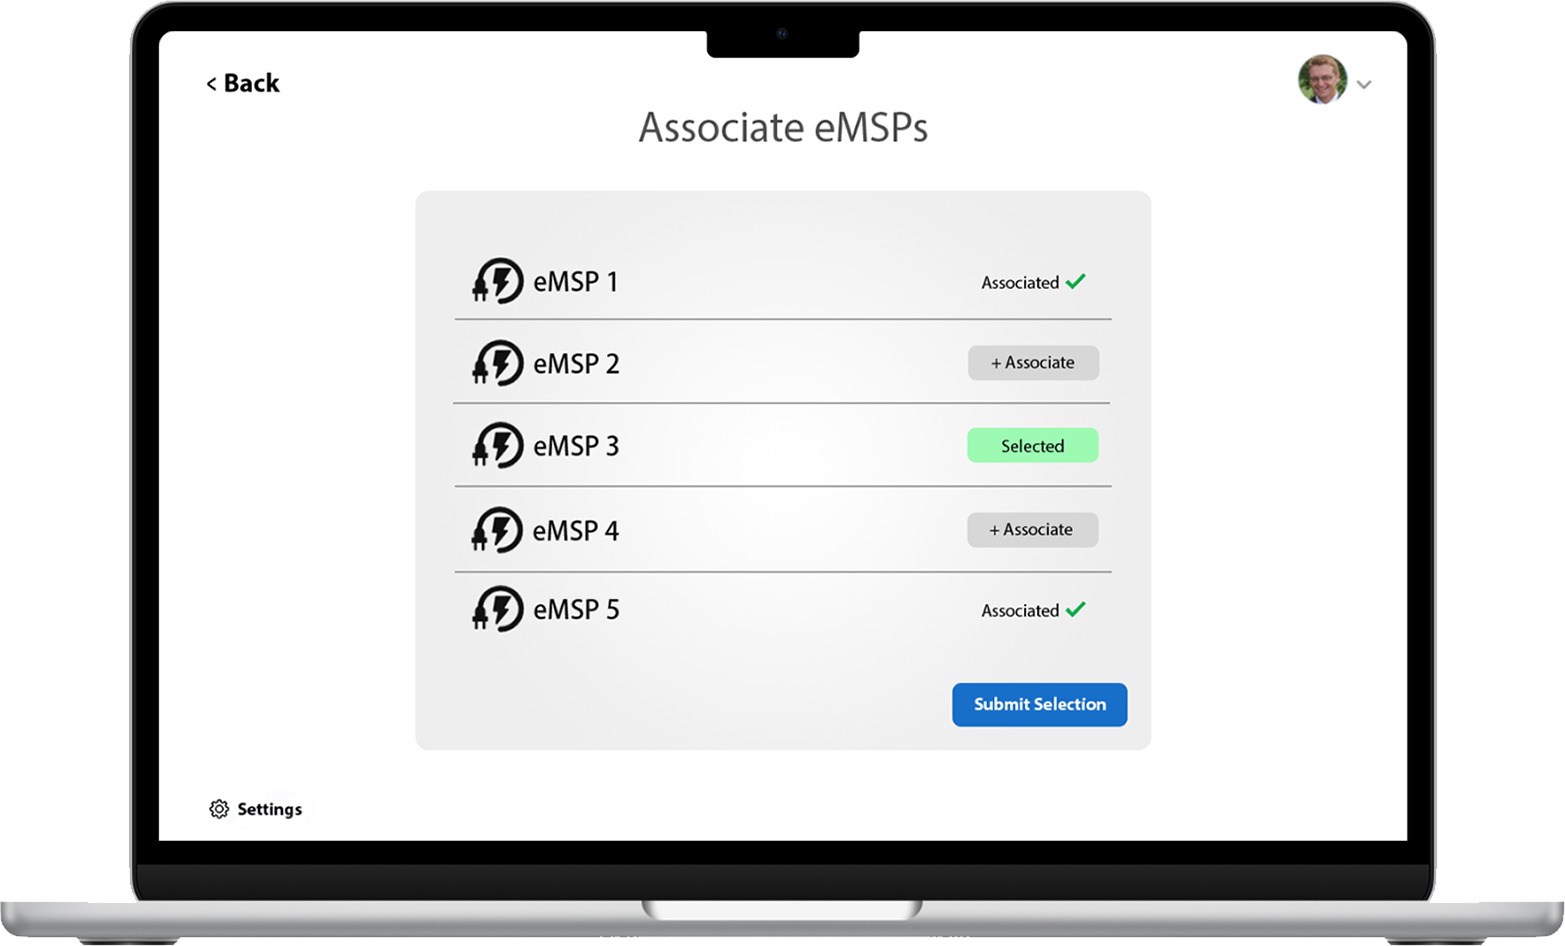
\includegraphics[
        width=\textwidth,
        height=\textheight,
        keepaspectratio]{Mock/CPMS/AssociateeMSP}
    \caption{Associate eMSPs Page}
    \label{fig:AssociateeMSP}
    \end{center}
\end{figure}
The mockup shows the eMSP association page, accessible from the main page, from which the CPO can select the eMSPs which he wants its CPMS to associate to. In the same page he can also see the already associated ones.